\documentclass[border=8pt,multi=tikzpicture]{standalone}
\usepackage{tikz}
\usetikzlibrary{positioning,fit,backgrounds,arrows.meta,shapes.geometric,calc}
\begin{document}

% ============================================================
% Figure 1 — Architecture
% ============================================================
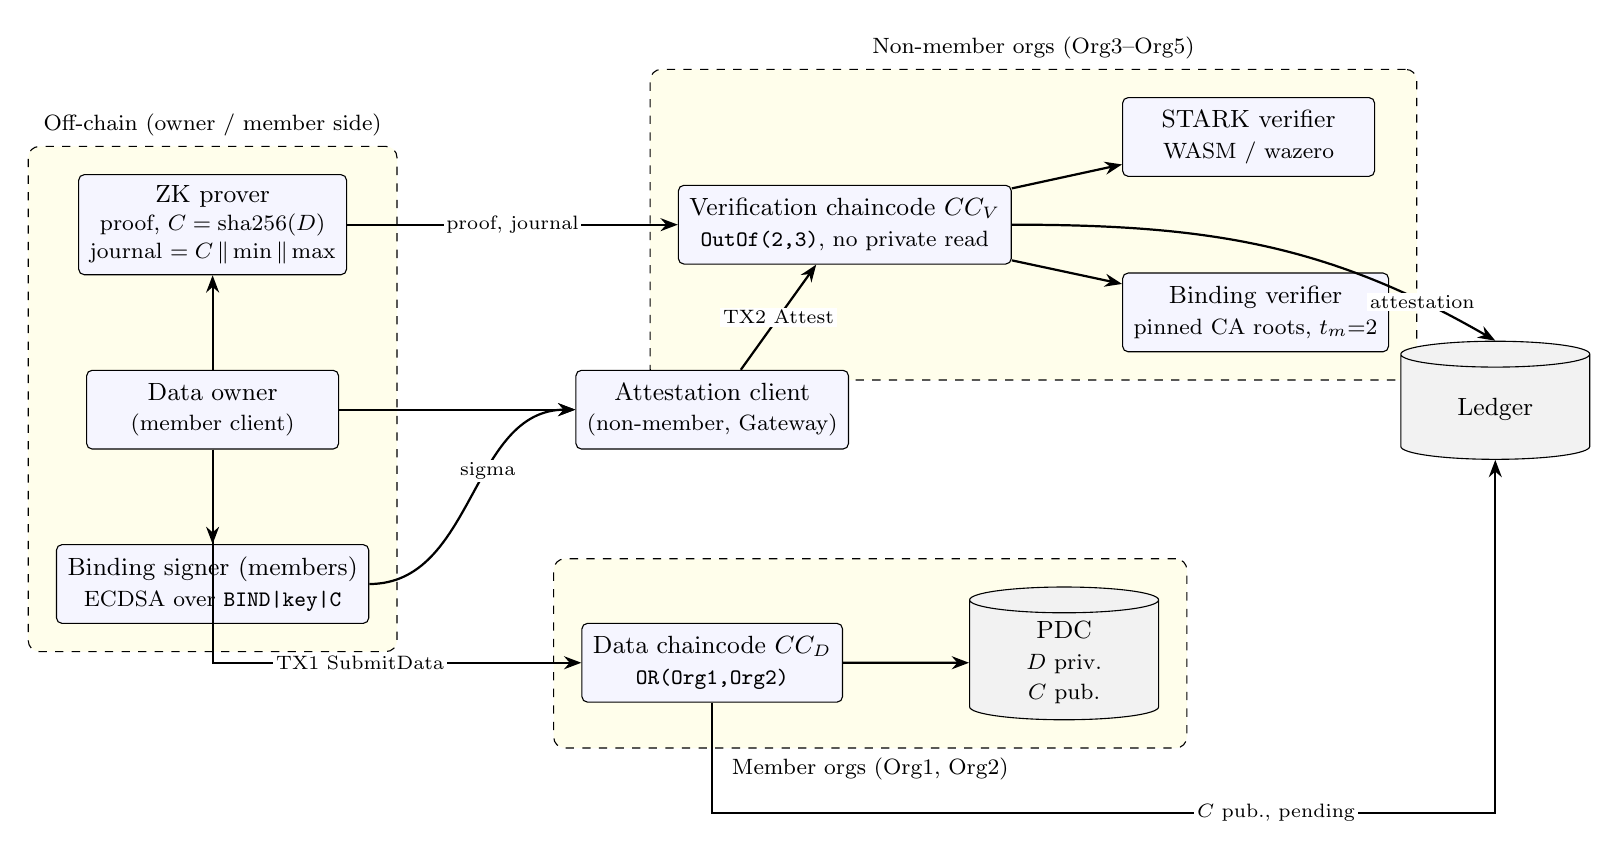
\begin{tikzpicture}[
  font=\small,
  box/.style={draw, rounded corners=2pt, align=center, inner sep=4pt,
              minimum height=10mm, minimum width=32mm, fill=blue!4},
  db/.style={draw, cylinder, shape border rotate=90, aspect=0.28, align=center,
             inner sep=3pt, fill=black!5, minimum height=15mm, minimum width=24mm},
  grp/.style={draw, dashed, rounded corners=4pt, inner sep=10pt, fill=yellow!8},
  arr/.style={-{Stealth[length=2.2mm]}, thick},
  lbl/.style={font=\scriptsize, fill=white, inner sep=1pt},
  node distance=12mm and 30mm]

  % --- off-chain column ---
  \node[box] (prover) {ZK prover\\[-1pt]\footnotesize proof, $C=\mathrm{sha256}(D)$\\[-1pt]\footnotesize journal $=C\,\|\min\|\max$};
  \node[box, below=of prover] (owner) {Data owner\\\footnotesize (member client)};
  \node[box, below=of owner] (signer) {Binding signer (members)\\\footnotesize ECDSA over \texttt{BIND|key|C}};

  % --- non-members ---
  \node[box, right=42mm of prover] (ccv) {Verification chaincode $CC_V$\\\footnotesize \texttt{OutOf(2,3)}, no private read};
  \node[box, above right=1mm and 14mm of ccv] (ver) {STARK verifier\\\footnotesize WASM / wazero};
  \node[box, below right=1mm and 14mm of ccv] (bnd) {Binding verifier\\\footnotesize pinned CA roots, $t_m{=}2$};

  % --- client ---
  \node[box, right=30mm of owner] (client) {Attestation client\\\footnotesize (non-member, Gateway)};

  % --- members ---
  \node[box, below=22mm of client] (ccd) {Data chaincode $CC_D$\\\footnotesize \texttt{OR(Org1,Org2)}};
  \node[db, right=16mm of ccd] (pdc) {PDC\\\footnotesize $D$ priv.\\\footnotesize $C$ pub.};

  % --- ledger ---
  \node[db, right=70mm of client] (led) {Ledger};

  % --- edges ---
  \draw[arr] (owner) -- (prover);
  \draw[arr] (owner) -- (signer);
  \draw[arr] (owner) -- (client);
  \draw[arr] (prover) -- (ccv) node[lbl,pos=0.5]{proof, journal};
  \draw[arr] (signer.east) to[out=0,in=180] node[lbl,pos=0.6]{sigma} (client.west);
  \draw[arr] (client) -- (ccv) node[lbl,pos=0.5]{TX2 Attest};
  \draw[arr] (ccv) -- (ver);
  \draw[arr] (ccv) -- (bnd);
  \draw[arr] (owner.south) |- (ccd.west) node[lbl,pos=0.7]{TX1 SubmitData};
  \draw[arr] (ccd) -- (pdc);
  \draw[arr] (ccd.south) -- ++(0,-1.4) coordinate (pc) -| (led.south);
  \node[lbl] at ($(pc)!0.72!(pc-|led.south)$) {$C$ pub., pending};
  \draw[arr] (ccv.east) to[out=0,in=150] node[lbl,pos=0.85]{attestation} (led.north);

  % --- group frames ---
  \begin{scope}[on background layer]
    \node[grp, fit=(prover)(owner)(signer), label={[font=\footnotesize]above:Off-chain (owner / member side)}] {};
    \node[grp, fit=(ccv)(ver)(bnd), label={[font=\footnotesize]above:Non-member orgs (Org3--Org5)}] {};
    \node[grp, fit=(ccd)(pdc), label={[font=\footnotesize]below:Member orgs (Org1, Org2)}] {};
  \end{scope}
\end{tikzpicture}

% ============================================================
% Figure 2 — Sequence
% ============================================================
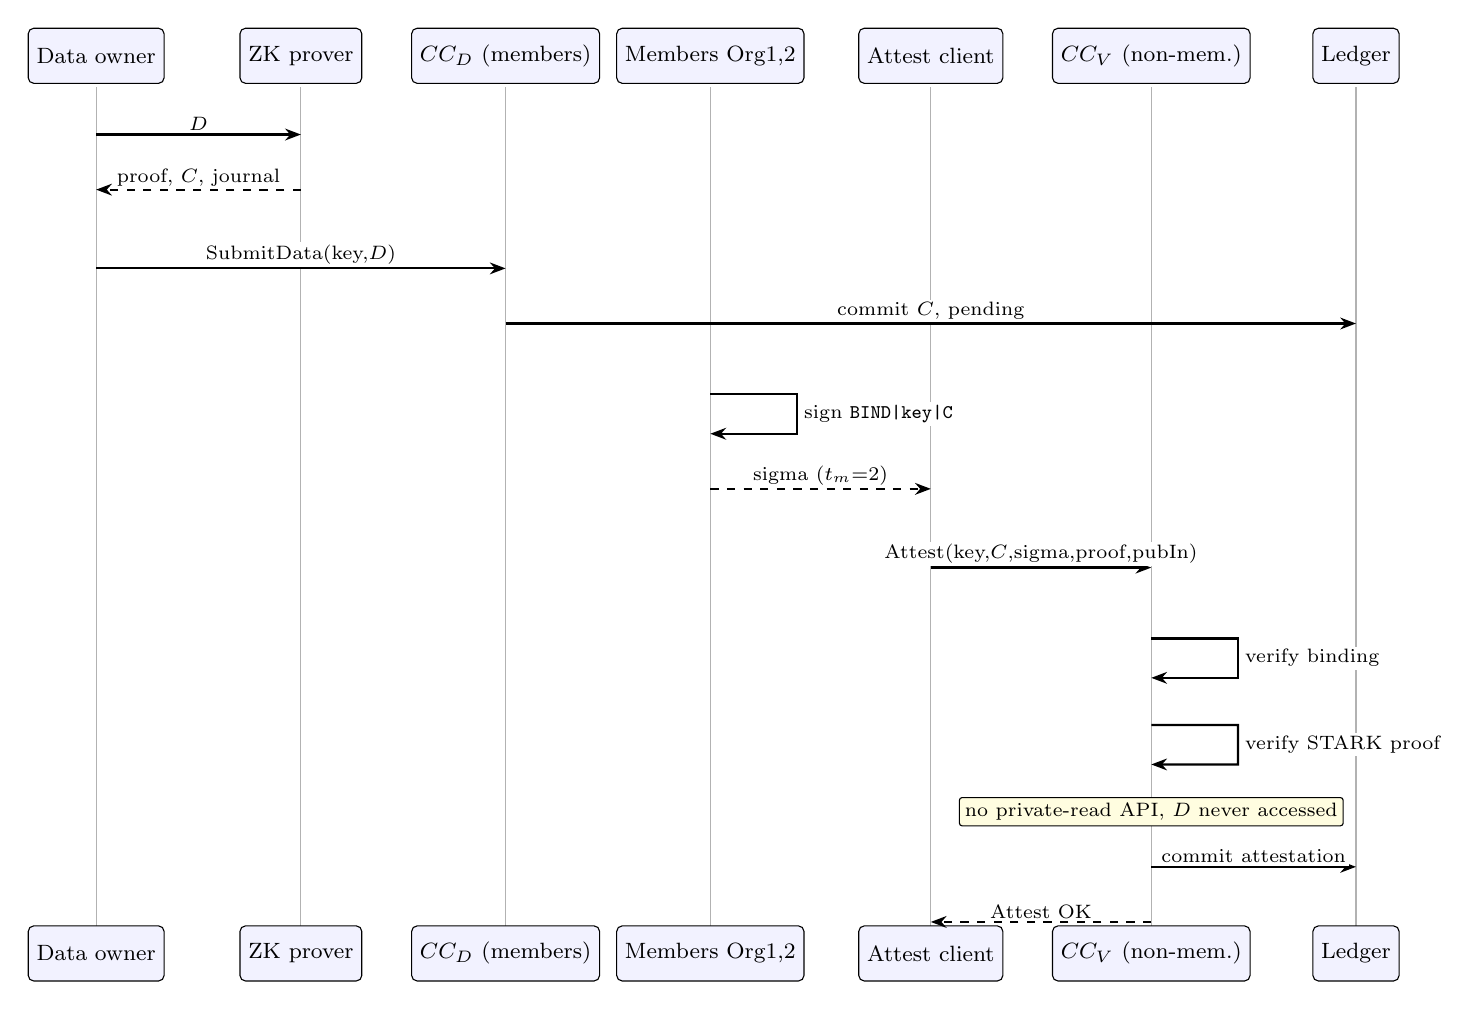
\begin{tikzpicture}[
  font=\footnotesize,
  head/.style={draw, rounded corners=2pt, fill=blue!5, align=center, inner sep=3pt, minimum height=7mm},
  msg/.style={-{Stealth[length=2mm]}, thick},
  ret/.style={-{Stealth[length=2mm]}, thick, dashed},
  note/.style={draw, fill=yellow!12, rounded corners=1pt, font=\scriptsize, inner sep=2pt},
  ml/.style={font=\scriptsize, fill=white, inner sep=1pt}]

  \def\ytop{0}\def\ybot{-11.4}
  \foreach \n/\x/\t in {O/0/{Data owner},P/2.6/{ZK prover},D/5.2/{$CC_D$ (members)},M/7.8/{Members Org1,2},S/10.6/{Attest client},V/13.4/{$CC_V$ (non-mem.)},L/16/{Ledger}}{
    \node[head] (\n) at (\x,\ytop) {\t};
    \draw[gray!60] (\x,-0.4) -- (\x,\ybot);
    \node[head] at (\x,\ybot) {\t};
  }

  \draw[msg] (0,-1.0) -- node[ml,above]{$D$} (2.6,-1.0);
  \draw[ret] (2.6,-1.7) -- node[ml,above]{proof, $C$, journal} (0,-1.7);

  \draw[msg] (0,-2.7) -- node[ml,above]{SubmitData(key,$D$)} (5.2,-2.7);
  \draw[msg] (5.2,-3.4) -- node[ml,above]{commit $C$, pending} (16,-3.4);

  \draw[msg] (7.8,-4.3) -- ++(1.1,0) -- ++(0,-0.5) -- (7.8,-4.8);
  \node[ml, right] at (8.95,-4.55){sign \texttt{BIND|key|C}};
  \draw[ret] (7.8,-5.5) -- node[ml,above]{sigma ($t_m{=}2$)} (10.6,-5.5);

  \draw[msg] (10.6,-6.5) -- node[ml,above]{Attest(key,$C$,sigma,proof,pubIn)} (13.4,-6.5);

  \draw[msg] (13.4,-7.4) -- ++(1.1,0) -- ++(0,-0.5) -- (13.4,-7.9);
  \node[ml,right] at (14.55,-7.65){verify binding};
  \draw[msg] (13.4,-8.5) -- ++(1.1,0) -- ++(0,-0.5) -- (13.4,-9.0);
  \node[ml,right] at (14.55,-8.75){verify STARK proof};
  \node[note] at (13.4,-9.6) {no private-read API, $D$ never accessed};

  \draw[msg] (13.4,-10.3) -- node[ml,above]{commit attestation} (16,-10.3);
  \draw[ret] (13.4,-11.0) -- node[ml,above]{Attest OK} (10.6,-11.0);
\end{tikzpicture}

\end{document}
